% HW5 Report Outline
\documentclass{article}
\usepackage{amsmath}
\usepackage{graphicx}
\usepackage{float}
\usepackage{hyperref}
% Add this to your LaTeX document preamble:
\usepackage{tikz}
\usetikzlibrary{shapes.geometric, arrows.meta, positioning}

\title{HW5: KNN Classification}
\author{Thomas Meltesen}
\date{2/26/2026}

\begin{document}

\maketitle

\section{Introduction}
Experiment with KNN-based classification using Python in combination with in
lecture discussed ML, data processing, and data visualization packages. With data from \texttt{HW05\textunderscore data.csv}:
% a) Loading the HW05_data.csv dataset
\begin{table}[ht]
\centering
\begin{tabular}{|c|c|c|}
\hline
Set & X Shape & Y Shape \\
\hline
Main Data   & (569, 30) & (569, 1) \\
\hline
\end{tabular}
\caption{HW5 Data}
\label{tab:data_split}
\end{table}



\section{Model Design}
% c) Splitting data into development and test sets
The model follows this basic outline, further explanation of the step implementations is further expanded on in section three.
% In your document:
\begin{figure}[H]
\centering
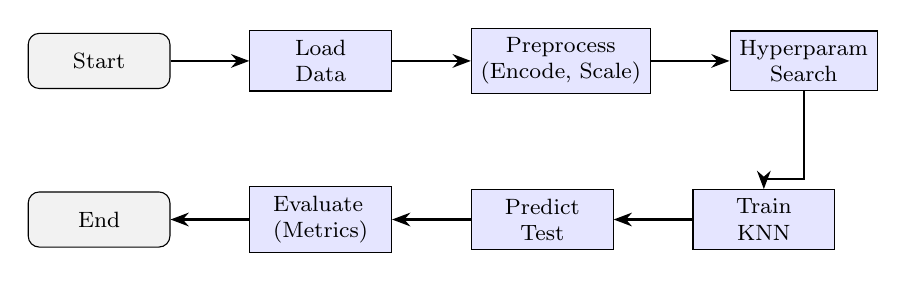
\begin{tikzpicture}[node distance=1.3cm and 1cm, every node/.style={font=\footnotesize}]
\tikzstyle{startstop} = [rectangle, rounded corners, minimum width=1.8cm, minimum height=0.7cm, text centered, draw=black, fill=gray!10]
\tikzstyle{process} = [rectangle, minimum width=1.8cm, minimum height=0.7cm, text centered, draw=black, fill=blue!10]
\tikzstyle{arrow} = [thick,->,>=Stealth]

% First row (top) - left to right
\node (start) [startstop] {Start};
\node (load) [process, right=of start, align=center] {Load\\Data};
\node (prep) [process, right=of load, align=center] {Preprocess\\(Encode, Scale)};
\node (search) [process, right=of prep, align=center] {Hyperparam\\Search};

% Second row (bottom) - right to left (reversed positions)
\node (end) [startstop, below=of start] {End};
\node (eval) [process, right=of end, align=left] {Evaluate\\(Metrics)};
\node (predict) [process, right=of eval, align=center] {Predict\\Test};
\node (train) [process, right=of predict, align=center] {Train\\KNN};

% First row arrows (left to right)
\draw [arrow] (start) -- (load);
\draw [arrow] (load) -- (prep);
\draw [arrow] (prep) -- (search);

% Arrow down from search to train
\draw [arrow] (search) -- ++(0,-1.5) -| (train);

% Second row arrows (right to left)
\draw [arrow] (train) -- (predict);
\draw [arrow] (predict) -- (eval);
\draw [arrow] (eval) -- (end);

\end{tikzpicture}
\caption{KNN System Design Flowchart}
\label{fig:knn_flowchart}
\end{figure}

\section{Training}

\subsection{Preprocessing}
% Preprocessing steps
For pre-processing, I process the data in these steps:
\begin{itemize}
    \item[1)]  Encode all variables of Y into representative numbers that our ML model can use. Using sklearns preprocessing package I take the 569 categorical labels of benign and malignant. And convert to their respective binary labels so the downstream ML algorithms can make use of the information.
    \item[2)] I assign a random state equal to 42 then run stratified train test splits as defined in the tables below \ref{tab:data_split} and \ref{tab:stratify} using sklearns train test split function.
    \item[3)]  I standardize the development and test data so that $\mu=0$ and its $\sigma=1$ via Standard Scaler.
\end{itemize}
The 569 sample dataset from the Homework 5 csv:
% Table: Data Split Summary
\begin{table}[ht]
\centering
\begin{tabular}{|c|c|c|}
\hline
Set & X Shape & Y Shape \\
\hline
Development (75\%)   & (426, 30) & (426, 1) \\
Test (25\%)       & (143, 30) & (143, 1) \\
\hline
\end{tabular}
\caption{Data Split: Development and Test Sets}
\label{tab:data_split}
\end{table}

This data is then stratified to ensure an accurate representation of both classes into these respective amounts.

\begin{table}[h!]
\centering
\begin{tabular}{lcc}
\hline
 & Test Set & Train Set \\
\hline
Class: Benign & 90 & 267 \\
Class: Malignant  & 53 & 159 \\
\hline
\end{tabular}
\caption{Stratified class distribution in train and test sets}
\label{tab:stratify}
\end{table}
\subsection{Hyperparameter Optimization and Cross-Validation}
% Searching for optimal K
I consider the following hyperparameters for the KNN classifier due to their inherent influence on the models performance:
\begin{itemize}
    \item \textbf{K}: Number of neighbors to consider.
    \item \textbf{p}: Distance metric, where $p=1$ corresponds to Manhattan distance, $p=2$ to Euclidean distance, and $p=3,4,5$ to higher-order Minkowski distances.
    \item \textbf{weights}: The weight function used in prediction, either \texttt{'uniform'} (all neighbors equally weighted) or \texttt{'distance'} (closer neighbors have greater influence).
\end{itemize}

I use these hyperparameter values in a Stratified 5-fold inside \texttt{GridSearchCV} to search for the optimal parameters for the KNN classifier. I chose the Stratified 5 fold as it is the most common number of folds that works well for most ML applications as well it provides accurate representation for both classes across folds. The optimal set is determined by cross-validating on the development set and selecting the configuration with the highest F1 score, which I chose due to its robustness across precision and recall. After optimizing these hyper parameters, the best parameters I found were: \textbf{K} = 3, \textbf{p} = 1, \textbf{weights} = 'uniform'.

So finally, once optimization was complete, I retrained the KNN classifier model on strictly the development set. Then after training I fed the test set into the model and the resulting performance metrics I found are referenced in \ref{tab:report}.

\section{Results}
\subsection{Performance Metrics}
%d) Performance metrics and evaluation
\begin{table}[H]
	\centering
	\caption{Classification Report for KNN Classifier}
	\begin{tabular}{lcccc}
		\hline
		& Precision & Recall & F1-score & Support \\
		\hline
		Benign & 0.96 & 1.00 & 0.98 & 90 \\
		Malignant & 1.00 & 0.92 & 0.96 & 53 \\
		\hline
		Accuracy & & & 0.97 & 143 \\
		Macro avg & 0.98 & 0.96 & 0.97 & 143 \\
		Weighted avg & 0.97 & 0.97 & 0.97 & 143 \\
		\hline
	\end{tabular}
	\label{tab:report}
\end{table}

Based on this classification report, the model performs well in classifying the two classes. This is evident from the high precision, recall, and F1 scores, all of which are close to 1. High precision indicates that the model rarely raises false alarms, while high recall shows that it rarely misses cases. The F1 score, being the harmonic mean of precision and recall, confirms that the model achieves a good balance between minimizing missed cases and false positives.

\subsection{Confusion Matrix}
\begin{figure}[h!]
	\centering
	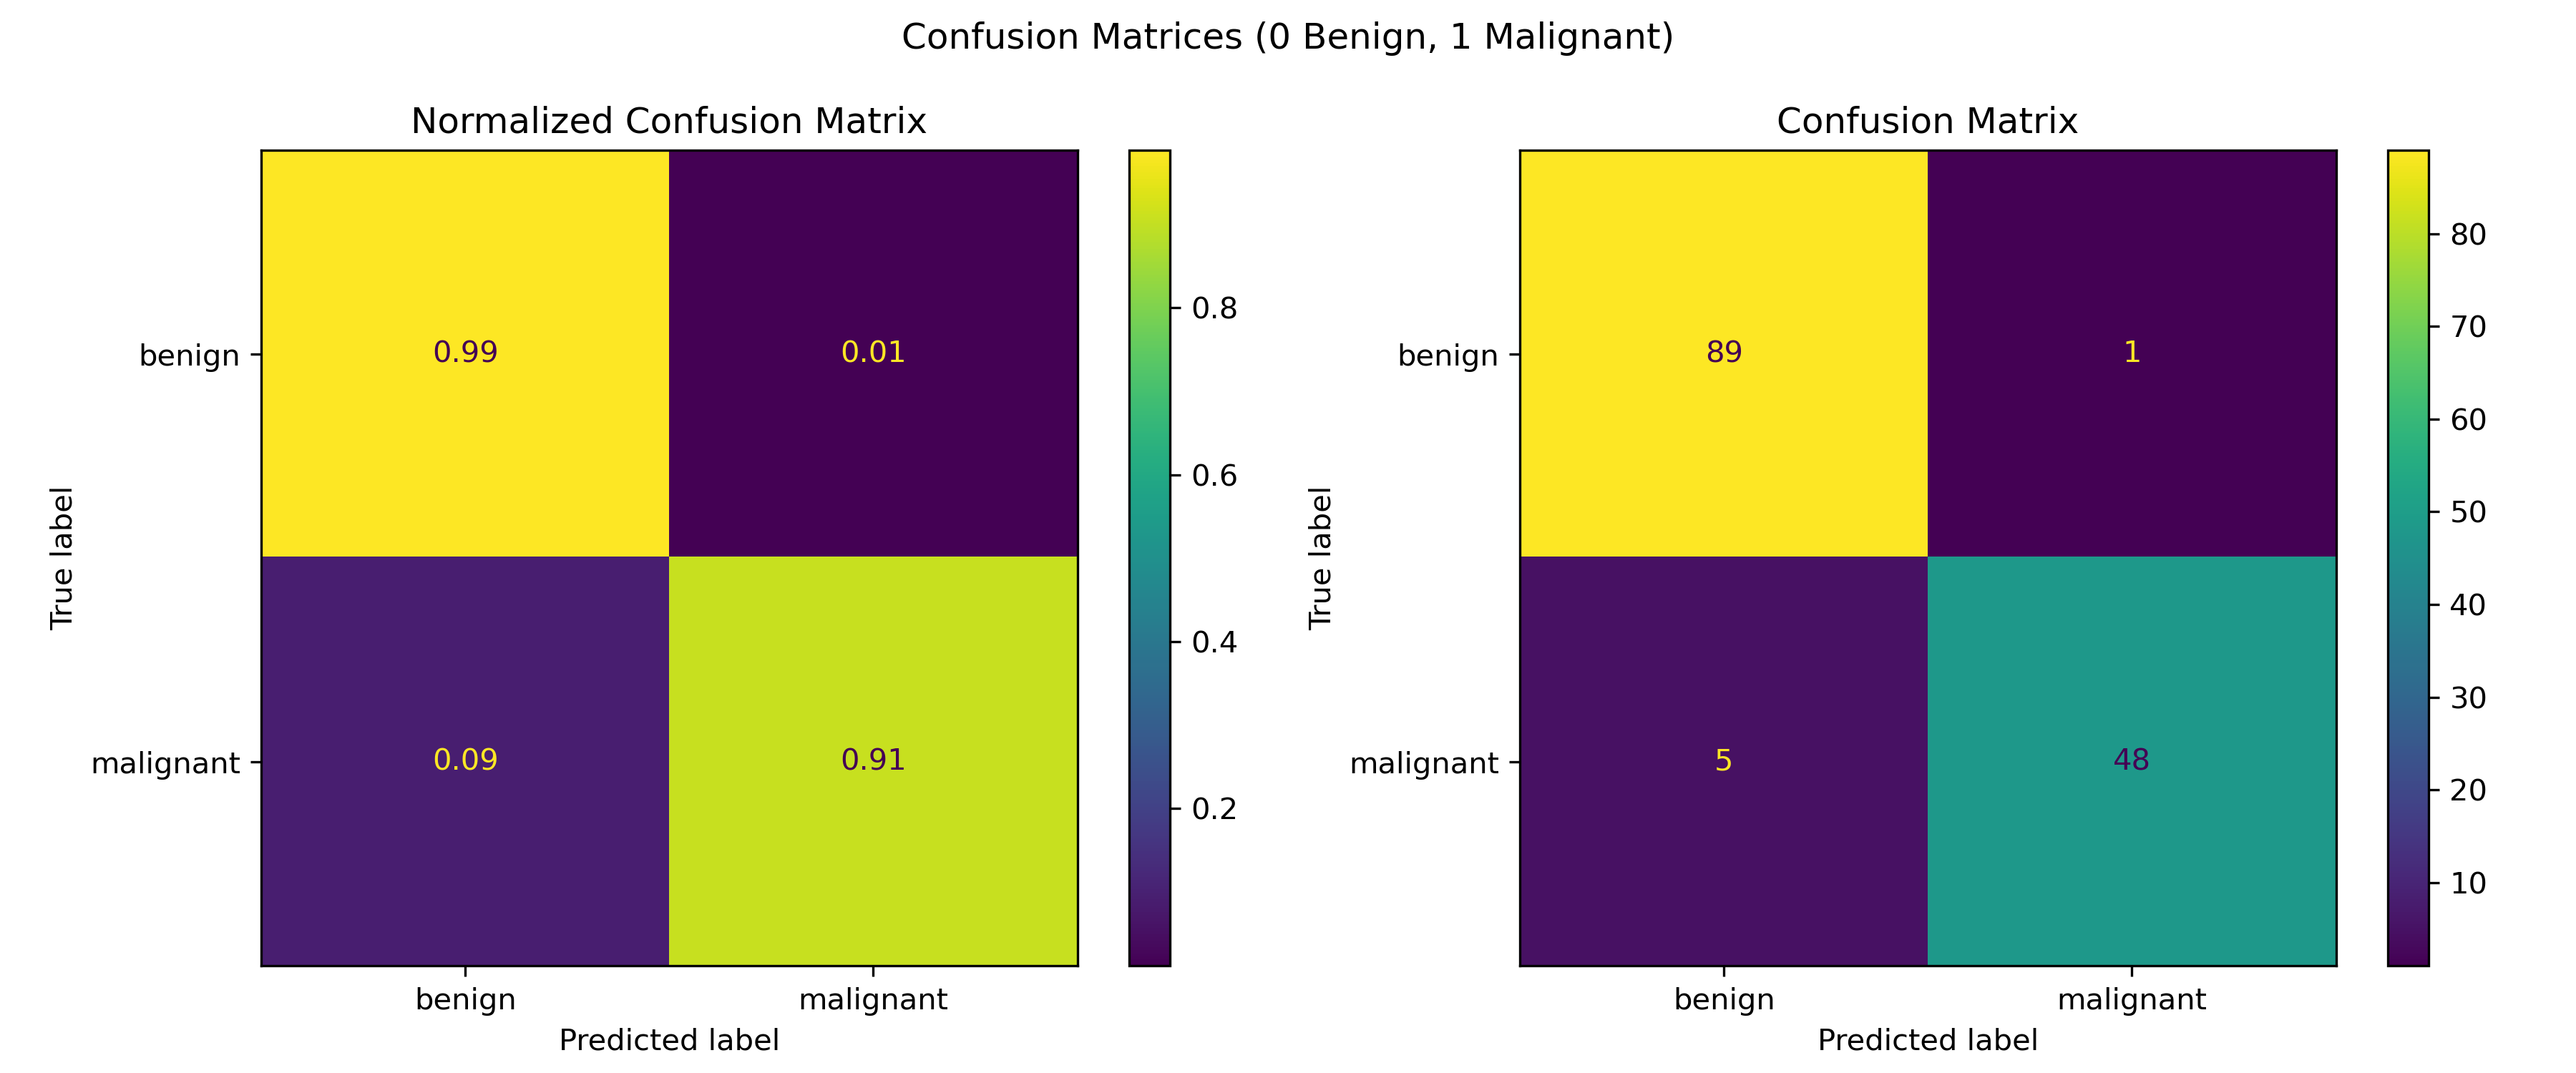
\includegraphics[width=1.1\textwidth]{knn_confusion_matrix.png}
	\caption{Confusion matrix for KNN classifier on test set.}
	\label{fig:knn_confusion_matrix}
\end{figure}

The confusion matrix further supports these findings, showing that the model achieves approximately 97 percent test accuracy and reliably classifies both classes. Most predictions are correct, with only a small number of misclassifications, indicating the model is effective for this dataset.

\section{Conclusion}
% Summary and final thoughts

 In conclusion, the KNN classifier, which was optimized through cross-validation and hyperparameter tuning, demonstrates strong performance on the dataset. The model achieves high precision, recall, and F1 scores for both benign and malignant classes, with an overall test accuracy of approximately 97 percent. The confusion matrix confirms that the misclassifications are minimal. Future work could explore additional pre-processing techniques or alternative classifiers to further optimize performance across random states since this only concerns one random state. But overall, like mentioned before future work can be done to research alternatives or further improve the classification performance.

\section{Disclaimers}
\begin{itemize}
    \item All Python code for data processing, model training, and visualization is available in the Jupyter notebook (\texttt{hw5.ipynb}).
    
\item This LaTeX document was formatted and generated by AI. All data, images and text were written in spaces by me to provide for a properly formatted report and ensure readability.

\item When writing the program, Copilot supports auto-complete which was used in some function writing.
\end{itemize}
 
\end{document}
